\documentclass[11pt]{article}

\usepackage[margin=1in]{geometry}
\usepackage{amsmath,amssymb}
\usepackage{graphicx}
\usepackage{booktabs}
\usepackage{xcolor}
\usepackage{listings}
\usepackage[colorlinks=true,linkcolor=blue,citecolor=blue,urlcolor=blue]{hyperref}

\lstset{
  basicstyle=\ttfamily\small,
  keywordstyle=\color{blue!60!black},
  commentstyle=\color{green!40!black}\itshape,
  numberstyle=\tiny\color{gray},
  showstringspaces=false,
  breaklines=true,
  frame=single,
  framesep=4pt,
  rulecolor=\color{gray!50},
  captionpos=b,
}
\lstdefinestyle{f90}{language=[90]Fortran}

\newcommand{\code}[1]{\texttt{#1}}
\newcommand{\sigeff}{\bar{\sigma}}
\newcommand{\sigtot}{\Sigma}

\title{Effective normal stress in HBI: governing equations, the\\
       \code{limitsigma} implementation, and a state-corrupting clamp}
\author{Notes for job 632510 (Cooper Basin / Habanero)}
\date{31 July 2026}

\begin{document}
\sloppy
\maketitle

\begin{abstract}
\noindent
The cumulative-slip profile of job 632510 has a local \emph{minimum} at the
injection point rather than a maximum. This document (i) writes out the
physics HBI solves and how it is discretised, (ii) shows that the
\code{limitsigma} floor on effective normal stress is applied in a way that
writes back into the stored state, so that the total normal stress ratchets
upward without bound, (iii) verifies against the job~632510 output that the
stored total normal stress equals $\sigma_{\min}+\max_t p$ to within
$6\times10^{-3}$~MPa in every cell that ever hit the floor, and (iv) explains
why a $115$~MPa error in normal stress produces only a $1.1$~cm signature in
slip. A patch is proposed in \S\ref{sec:fix}.
\end{abstract}

\tableofcontents

%======================================================================
\section{Scope and conventions}

Everything below refers to \code{problem 3dp}: a planar rectangular fault
discretised into $i_{\max}\times j_{\max}$ uniform square cells, with
along-fault fluid-pressure diffusion switched on
(\code{pressurediffusion T}). Line numbers refer to the working tree at the
time of writing.

HBI uses a mixed unit system; getting this right matters for reading the
source. Table~\ref{tab:units} lists the conventions actually used in
\code{main\_LH.f90} and \code{m\_diffusion.f90}.

\begin{table}[h]
\centering
\begin{tabular}{lll}
\toprule
Quantity & Unit & Notes \\
\midrule
stress ($\tau,\sigma,p$)         & MPa   & \code{sigmainit 30.0} is 30~MPa \\
length (\code{ds}, \code{xcol})  & km    & \code{ds 0.005} is a 5~m cell \\
slip                              & m     & \\
slip rate                         & m/s   & \code{vref}$=10^{-6}$ (l.\,150) \\
time                              & s     & \code{tmax} is in years, converted on read \\
rigidity \code{rigid}             & GPa   & \code{rigid 24} \\
shear wave speed \code{vs}        & km/s  & default $3.464$ \\
permeability \code{kp}            & m$^2$ & \\
viscosity \code{eta}              & Pa\,s & \\
compressibility \code{beta}       & Pa$^{-1}$ & \\
\bottomrule
\end{tabular}
\caption{Unit conventions. The mixed GPa/km/MPa choice is self-consistent:
e.g.\ $\code{rigid}/\code{vs}$ has units GPa/(km\,s$^{-1}$) $=$
MPa/(m\,s$^{-1}$), which is the correct unit for the radiation-damping
coefficient.}
\label{tab:units}
\end{table}

Throughout, $\sigeff$ denotes \emph{effective} normal stress and $\sigtot$
\emph{total} normal stress, related by Terzaghi's principle,
\begin{equation}
  \sigeff = \sigtot - p .
  \label{eq:terzaghi}
\end{equation}
In the code these are the arrays \code{sigma} and \code{sigmat} respectively,
and \code{pf} is $p$. Note that \code{sigma} --- despite the name --- is the
\emph{effective} normal stress; this is the single most common source of
confusion when reading \code{main\_LH.f90}.

%======================================================================
\section{Governing equations}

\subsection{Quasi-dynamic elasticity}

The fault is embedded in a homogeneous elastic half-space. Slip
$\delta(\mathbf{x},t)$ on the fault generates shear and normal traction
changes given by a boundary integral over the fault surface. Discretised on
$N$ cells, with $V_j=\dot\delta_j$,
\begin{equation}
  \dot\tau^{\rm el}_i = \sum_{j=1}^{N} K^{s}_{ij}\,(V_j - V_{\rm pl}),
  \qquad
  \dot\sigtot_i = \sum_{j=1}^{N} K^{n}_{ij}\,(V_j - V_{\rm pl}),
  \label{eq:bem}
\end{equation}
where $K^s$ and $K^n$ are the shear-shear and shear-normal stress-interaction
kernels. For rectangular cells these come from the Okada (1992) dislocation
solution (\code{okada.f90}, reached through
\code{HACApK\_entry\_ij} in \code{m\_HACApK\_calc\_entry\_ij.f90:61--63}).
The $V_{\rm pl}$ subtraction is the \code{backslip} formulation; this run sets
\code{vpl 0d0}, so there is no tectonic loading and all stressing comes from
the injection.

The dense matrices $K^s,K^n$ are never formed. They are compressed into
lattice $\mathcal{H}$-matrices by HACApK and applied as matrix--vector
products (\code{HACApK\_\allowbreak adot\_\allowbreak lattice\_\allowbreak hyp},
\code{main\_LH.f90:1852,1863}).

\paragraph{A planar fault has no self-induced normal stress change.}
For a planar fault, slip on the plane produces \emph{zero} change in the
normal traction on that same plane: $K^n\equiv 0$. The code recognises this
explicitly and skips the normal kernel entirely
(\code{main\_LH.f90:501--503}):
\begin{lstlisting}[style=f90]
  select case(problem)
  case('2dp','2dn3','3dp','2dvs')
    sigmaconst=.true.
  end select
\end{lstlisting}
so that for \code{3dp} the code sets $\dot\sigtot^{\rm el}=0$
(\code{main\_LH.f90:1860--1861}). \textbf{This is important for what follows:
in this run the total normal stress has no elastic contribution at all, so
$\sigtot$ must remain exactly $\sigma_{\rm init}=30$~MPa for all time, and the
effective normal stress must be exactly $30-p$.}

\subsection{The quasi-dynamic approximation}

Full elastodynamics is replaced by the radiation-damping approximation: the
inertial term is modelled by a local dashpot,
\begin{equation}
  \tau = \tau^{\rm el} - \eta V,
  \qquad
  \eta = \frac{\mu}{2 c_s},
  \label{eq:raddamp}
\end{equation}
with $\mu$ the shear modulus and $c_s$ the shear wave speed. In the code
$\eta$ appears as \code{0.5d0*rigid/vs}.

\subsection{Rate-and-state friction}

Sliding obeys a regularised rate-and-state law. HBI carries the state as
$\psi$, a friction-like variable, and inverts the friction law for slip rate
(\code{main\_LH.f90:1820}):
\begin{equation}
  V = 2 V_{\rm ref}\,
      \exp\!\left(-\frac{\psi}{a}\right)
      \sinh\!\left(\frac{\tau}{a\,\sigeff}\right).
  \label{eq:vel}
\end{equation}
This is the standard regularisation of $\tau = \sigeff\,[\,f_0 + a\ln(V/V_0) +
b\ln(V_0\theta/d_c)\,]$, well behaved as $V\to0$ and for $V<0$.

The state evolves by the ageing law (\code{evlaw} defaults to \code{aging};
\code{main\_LH.f90:1924--1929}):
\begin{equation}
  \dot\psi = \frac{b\,V_{\rm ref}}{d_c}\exp\!\left(\frac{f_0-\psi}{b}\right)
             - \frac{b\,|V|}{d_c}.
  \label{eq:aging}
\end{equation}
This is exactly $\dot\theta = 1 - V\theta/d_c$ rewritten under the change of
variable $\psi = f_0 + b\ln(V_{\rm ref}\theta/d_c)$: differentiating gives
$\dot\psi = (b/\theta)\dot\theta = b/\theta - bV/d_c$, and
$b/\theta = (bV_{\rm ref}/d_c)\exp((f_0-\psi)/b)$.

Job 632510 uses $a=0.015$, $b=0.012$, so $a-b>0$: the fault is
velocity-\emph{strengthening} everywhere and slip is aseismic throughout.

\subsection{The evolution equation for shear stress}

Differentiating \eqref{eq:raddamp} and using
$V=V(\psi,\tau,\sigeff)$ from \eqref{eq:vel},
\begin{equation}
  \dot\tau = S - \eta\left(
    \frac{\partial V}{\partial \psi}\dot\psi
    + \frac{\partial V}{\partial \tau}\dot\tau
    + \frac{\partial V}{\partial \sigeff}\dot{\sigeff}
  \right),
  \qquad S \equiv \dot\tau^{\rm el},
\end{equation}
which solved for $\dot\tau$ gives, with $\dot{\sigeff} = \dot\sigtot - \dot p$,
\begin{equation}
  \boxed{\;
  \dot\tau =
  \frac{S - \eta\left[\dfrac{\partial V}{\partial\psi}\dot\psi
         + \dfrac{\partial V}{\partial\sigeff}\left(\dot\sigtot - \dot p\right)\right]}
       {1 + \eta\,\dfrac{\partial V}{\partial\tau}}\;}
  \label{eq:dtaudt}
\end{equation}
with partial derivatives obtained from \eqref{eq:vel},
\begin{equation}
  \frac{\partial V}{\partial\tau} = \frac{2V_{\rm ref}e^{-\psi/a}}{a\sigeff}
    \cosh\!\frac{\tau}{a\sigeff},
  \quad
  \frac{\partial V}{\partial\sigeff} = -\frac{2V_{\rm ref}e^{-\psi/a}\,\tau}
    {a\sigeff^{2}}\cosh\!\frac{\tau}{a\sigeff},
  \quad
  \frac{\partial V}{\partial\psi} = -\frac{V}{a}.
\end{equation}
Equation~\eqref{eq:dtaudt} is \code{main\_LH.f90:1963} verbatim; the partial
derivatives are lines 1960--1962. Note that the pore-pressure rate $\dot p$
enters only here, as a correction to the effective-stress rate.

\subsection{Fluid pressure diffusion}

Along-fault pressure obeys a linear diffusion equation with a heterogeneous,
slip-dependent diffusivity and a well source
(\code{m\_diffusion.f90}, \code{diffusion3dwop}/\code{Beuler2d}):
\begin{equation}
  \beta\phi\,\frac{\partial p}{\partial t}
  = \nabla\cdot\left(\frac{k}{\eta_f}\nabla p\right) + q ,
  \qquad
  c_{\rm hyd} = \frac{k}{\eta_f\,\beta\,\phi},
  \label{eq:diffusion}
\end{equation}
implemented as \code{cdiff = kpG/(eta*beta*phiG)*1d-6}
(\code{m\_diffusion.f90:443--445}; the $10^{-6}$ converts m$^2$/s to
km$^2$/s to match \code{ds0} in km). The scheme is backward Euler in time,
second order in space, solved with conjugate gradients; boundary conditions
are set by \code{bcl/bcr/bct/bcb} (all Dirichlet, $p=0$, in this run).

\paragraph{Permeability evolution.} With \code{permev T}
(\code{main\_LH.f90:2402--2405}),
\begin{equation}
  \frac{dk}{dt} = -\frac{V}{k_L}\left(k - k_{\max}\right)
                  - \frac{k - k_{\min}}{k_T},
  \label{eq:permev}
\end{equation}
i.e.\ slip enhances permeability toward $k_{\max}$ over a slip scale $k_L$,
and it heals back toward $k_{\min}$ over a time scale $k_T$. Job 632510 uses
$k_{\min}=10^{-15}$, $k_{\max}=5\times10^{-14}$~m$^2$, $k_L=10^{-3}$~m,
$k_T=10^{15}$~s (i.e.\ healing effectively disabled). The corresponding
hydraulic diffusivities are $c_{\rm hyd}\approx 5.6\times10^{-3}$~m$^2$/s
(intact) to $0.28$~m$^2$/s (fully enhanced).

\paragraph{Well source.} The injector is a single cell with a Peaceman
well-index coupling to a wellbore of radius $r_w$ with storage $S_w$
(\code{m\_diffusion.f90:669--675}):
\begin{equation}
  T = \frac{2\pi k}{\eta_f\left[\ln(0.2\,\Delta s/r_w) + s_{\rm skin}\right]},
  \qquad
  \gamma = \frac{S_w/\Delta t}{S_w/\Delta t + T},
\end{equation}
with the wellbore pressure updated as
$p_w^{n+1} = \gamma\left(p_w^{n} + \Delta t\, q/S_w\right)
             + (1-\gamma)\,p^{n+1}_{\rm cell}$
(\code{m\_diffusion.f90:763}). The injection schedule $q(t)$ is read from
\code{june\_clean.txt} and linearly interpolated between breakpoints.

\subsection{The coupled system}

Per cell the state vector is $y = (\psi,\ \tau,\ \sigeff)$, and the code
integrates
\begin{equation}
  \frac{d}{dt}
  \begin{pmatrix}\psi\\ \tau\\ \sigeff\end{pmatrix}
  =
  \begin{pmatrix}
    \text{\eqref{eq:aging}} \\[2pt]
    \text{\eqref{eq:dtaudt}} \\[2pt]
    \dot\sigtot^{\rm el}
  \end{pmatrix},
  \label{eq:ode}
\end{equation}
with an adaptive fifth-order Cash--Karp Runge--Kutta step (\code{rkqs},
\code{main\_LH.f90:1979}). Note the third component: within an RK step
$\sigeff$ is advanced by the \emph{elastic} normal-stress rate only. Pore
pressure is not integrated by the RK step at all --- it is handled by
operator splitting, described next.

%======================================================================
\section{How a timestep is assembled}
\label{sec:step}

One iteration of the main loop (\code{main\_LH.f90:1090--1135}) does:

\begin{enumerate}
\item \textbf{RK step.} \code{rkqs} advances $y$ over $\Delta t$ using
      \eqref{eq:ode}. Pore pressure is frozen at its old value; only $\dot p$
      from the previous step enters, through \eqref{eq:dtaudt}.
      (\code{main\_LH.f90:1091})

\item \textbf{Unpack and accumulate slip.} $\psi,\tau,\sigeff$ are copied out
      of $y$; slip is accumulated with a trapezoidal rule.
      (\code{main\_LH.f90:1102--1122})

\item \textbf{Reconstruct total normal stress.} (\code{main\_LH.f90:1124})
\begin{lstlisting}[style=f90]
      sigmat(i)=sigma(i)+pf(i)
\end{lstlisting}

\item \textbf{Diffusion step.} \code{pressure\_diffusion} advances
      \eqref{eq:permev} and \eqref{eq:diffusion} over the same $\Delta t$,
      then re-imposes Terzaghi's principle and applies the clamp
      (\code{main\_LH.f90:2449--2458}):
\begin{lstlisting}[style=f90]
      pf(i)=pfG(i_)
      dpdt(i)=(pf(i)-pfo(i))/dtdid
      sigma(i)=sigmat(i)-pf(i)
      if(limitsigma) then
        if(sigma(i)<minsig) sigma(i)=minsig
        if(sigma(i)>maxsig) sigma(i)=maxsig
      end if
      y(3*i)=sigma(i)
\end{lstlisting}
\end{enumerate}

The intent of the splitting is clear and correct: elasticity moves
$\sigtot$, diffusion moves $p$, and $\sigeff = \sigtot - p$ is reassembled
once per step. The defect is in how the clamp interacts with step 3.

%======================================================================
\section{The \code{limitsigma} clamp}

\subsection{What it is for}

Effective normal stress appears in the denominator of \eqref{eq:vel}. If
$\sigeff\to0$ the argument of $\sinh$ diverges; if $\sigeff<0$ the friction
law is meaningless (the fault would be in tension and should open). Runs in
which injection drives $p$ toward or past the ambient normal stress therefore
need some regularisation. HBI provides two:

\begin{itemize}
\item \code{opening T}: a physical treatment in which
      $\sigeff<\sigma_{\min}$ opens the fault, generating opening
      displacement that feeds back through the normal kernel
      (\code{main\_LH.f90:1838--1841}). This forces
      \code{sigmaconst=.false.} even for \code{3dp}.
\item \code{limitsigma T} (the default, and what job 632510 uses): a
      numerical floor, $\sigeff \leftarrow \max(\sigeff, \sigma_{\min})$.
\end{itemize}

A floor of this kind is defensible as a numerical safeguard \emph{provided it
is a pure projection}: it should modify the value handed to the friction law
without altering the underlying stress state. Under that reading, the correct
result is
\begin{equation}
  \sigeff(t) \;=\; \max\!\Big(\sigma_{\rm init} + \Delta\sigtot^{\rm el}(t) - p(t),\ \ \sigma_{\min}\Big),
  \label{eq:intended}
\end{equation}
which is a \emph{memoryless} function of the current $p$: as soon as $p$ falls
again, $\sigeff$ comes back up along $\sigma_{\rm init}-p$.

There is also a second, separate guard inside \code{deriv}
(\code{main\_LH.f90:1912--1916}) that zeroes $\dot\sigtot^{\rm el}$ when
$\sigeff$ is outside $[\sigma_{\min},\sigma_{\max}]$. That one is benign: it
suppresses a rate, it does not rewrite a state.

\subsection{The defect}

The clamped value written into \code{y(3*i)} at step 4 is read back at step 2
of the \emph{next} iteration and then, at step 3, added to $p$ to reconstruct
$\sigtot$. The clamp correction is therefore absorbed into the total normal
stress and becomes permanent. HBI has no independent record of $\sigtot$
against which to check this: \code{sigmat} is a derived quantity recomputed
from \code{sigma} every step, not a state variable.

%======================================================================
\section{Derivation of the ratchet}
\label{sec:derivation}

Index the operator-split steps by $n$, and for a single cell write
$\sigeff_n$, $p_n$, $\sigtot_n$ for the values of \code{sigma}, \code{pf},
\code{sigmat}. Let $\Delta_n = \int_{t_{n-1}}^{t_n}\dot\sigtot^{\rm el}\,dt$
be the elastic increment accumulated by RK step $n$ (identically zero for
\code{3dp}, since \code{sigmaconst=.true.}).

The four operations of \S\ref{sec:step} are
\begin{align}
  \text{(a) RK:}          &\quad \tilde\sigeff_n = \sigeff_{n-1} + \Delta_n
    &&\text{(l.\,1105)} \\
  \text{(b) reconstruct:} &\quad \sigtot_n = \tilde\sigeff_n + p_{n-1}
    &&\text{(l.\,1124)} \\
  \text{(c) diffuse:}     &\quad p_{n-1} \to p_n && \\
  \text{(d) re-impose:}   &\quad \sigeff^{\rm raw}_n = \sigtot_n - p_n
    &&\text{(l.\,2452)} \\
  \text{(e) clamp:}       &\quad \sigeff_n = \mathrm{clamp}\big(\sigeff^{\rm raw}_n\big)
    &&\text{(l.\,2454--2455)}
\end{align}

Composing (a), (b), (d):
\begin{equation}
  \sigeff^{\rm raw}_n = \sigeff_{n-1} + \Delta_n - (p_n - p_{n-1}).
\end{equation}
Define the clamp excess $e_n \equiv \sigeff_n - \sigeff^{\rm raw}_n$, which is
zero on unclamped steps and positive whenever the floor bites. Then
$\sigeff_n = \sigeff_{n-1} + \Delta_n - (p_n - p_{n-1}) + e_n$, and
telescoping from $n=0$:
\begin{equation}
  \boxed{\;
  \sigeff_N \;=\;
  \underbrace{\sigma_{\rm init} + \sum_{n\le N}\Delta_n - (p_N - p_0)}_{\text{correct}}
  \;+\;
  \underbrace{\sum_{n\le N} e_n}_{\text{accumulated clamp defect}} \; }
  \label{eq:telescope}
\end{equation}

Compare with the intended behaviour \eqref{eq:intended}. The correct result
depends only on the \emph{current} $p$; the implemented result carries the
sum of every clamp correction ever applied. That sum never decays.

\subsection{Closed form for a planar fault}

Set $\Delta_n\equiv0$ (true for \code{3dp}). Then from (b),
$\sigtot_n = \sigeff_{n-1} + p_{n-1}$, and two cases arise:

\begin{itemize}
\item \emph{Step $n-1$ was not clamped.} Then
      $\sigeff_{n-1} = \sigtot_{n-1} - p_{n-1}$, so
      $\sigtot_n = \sigtot_{n-1}$: unchanged, as it should be.
\item \emph{Step $n-1$ hit the floor.} Then $\sigeff_{n-1}=\sigma_{\min}$ and
      $\sigtot_n = \sigma_{\min} + p_{n-1}$. But hitting the floor means
      $\sigtot_{n-1} - p_{n-1} < \sigma_{\min}$, i.e.
      $\sigma_{\min} + p_{n-1} > \sigtot_{n-1}$. So $\sigtot$ has
      \emph{strictly increased}.
\end{itemize}

$\sigtot$ is therefore non-decreasing, and increases exactly at the pressure
peaks that trigger the floor. Hence, for any cell in which the floor was ever
reached,
\begin{equation}
  \boxed{\;\sigtot_{\rm final} \;=\; \sigma_{\min} + \max_{t}\,p(t)\;}
  \label{eq:ratchet}
\end{equation}
and for a cell that never reached the floor, $\sigtot_{\rm final} =
\sigma_{\rm init}$ exactly. Equivalently, the effective normal stress reported
by the code after the pressure has receded is
\begin{equation}
  \sigeff_{\rm code}(t) = \sigma_{\min} + \max_{t'\le t} p(t') - p(t)
  \quad\text{instead of}\quad
  \sigeff_{\rm true}(t) = \max\big(\sigma_{\rm init}-p(t),\ \sigma_{\min}\big).
  \label{eq:err}
\end{equation}

The floor bites when $p > \sigma_{\rm init} - \sigma_{\min}$, which for
job 632510 is $p > 29$~MPa.

%======================================================================
\section{Verification against job 632510}

Run \code{docs/verify\_clamp\_ratchet.py} to regenerate everything in this
section. Grid $601\times601$, $\Delta s = 5$~m, $\sigma_{\rm init}=30$~MPa,
$\sigma_{\min}=1$~MPa, injector at Fortran $(301,301)$, $1402$ output frames
spanning $30.66$~days.

\subsection{The ratchet identity}

Table~\ref{tab:ratchet} tests \eqref{eq:ratchet} cell by cell along a profile
through the injector.

\begin{table}[h]
\centering
\begin{tabular}{rrrrr}
\toprule
$j$ & $r$ (m) & $\max_t p$ & $\sigtot_{\rm final}$ & $\sigma_{\min}+\max_t p$ \\
\midrule
300 &   0 & 144.00 & 145.01 & 145.00 \\
305 &  25 &  71.12 &  72.12 &  72.12 \\
310 &  50 &  55.61 &  56.61 &  56.61 \\
317 &  85 &  44.04 &  45.04 &  45.04 \\
325 & 125 &  36.51 &  37.51 &  37.51 \\
340 & 200 &  28.47 &  \textbf{30.00} & 29.47 \\
360 & 300 &  21.79 &  \textbf{30.00} & 22.79 \\
400 & 500 &  14.22 &  \textbf{30.00} & 15.22 \\
450 & 750 &  10.02 &  \textbf{30.00} & 11.02 \\
\bottomrule
\end{tabular}
\caption{Stress in MPa. Cells with $\max_t p > 29$~MPa satisfy
\eqref{eq:ratchet}; cells that never reached the floor retain
$\sigtot=\sigma_{\rm init}=30.0000$ exactly (bold). Maximum residual
$|\sigtot - (\sigma_{\min}+\max_t p)|$ over all clamped cells:
$5.8\times10^{-3}$~MPa, attributable to output frames subsampling the
timesteps, so $\max_t p$ over frames slightly underestimates the true
maximum.}
\label{tab:ratchet}
\end{table}

The agreement is not approximate --- it is the identity derived in
\S\ref{sec:derivation}, holding to five significant figures, with a sharp
transition at exactly the predicted threshold. The clamped region is
$|r|\le190$~m.

At the injector the consequence is severe: $p$ peaks at $144$~MPa against an
ambient normal stress of $30$~MPa, so $\sigtot$ ends at $145$~MPa and the
reported effective normal stress reaches $135$~MPa --- a $115$~MPa error, more
than four times the true total normal stress.

\begin{figure}[h]
\centering
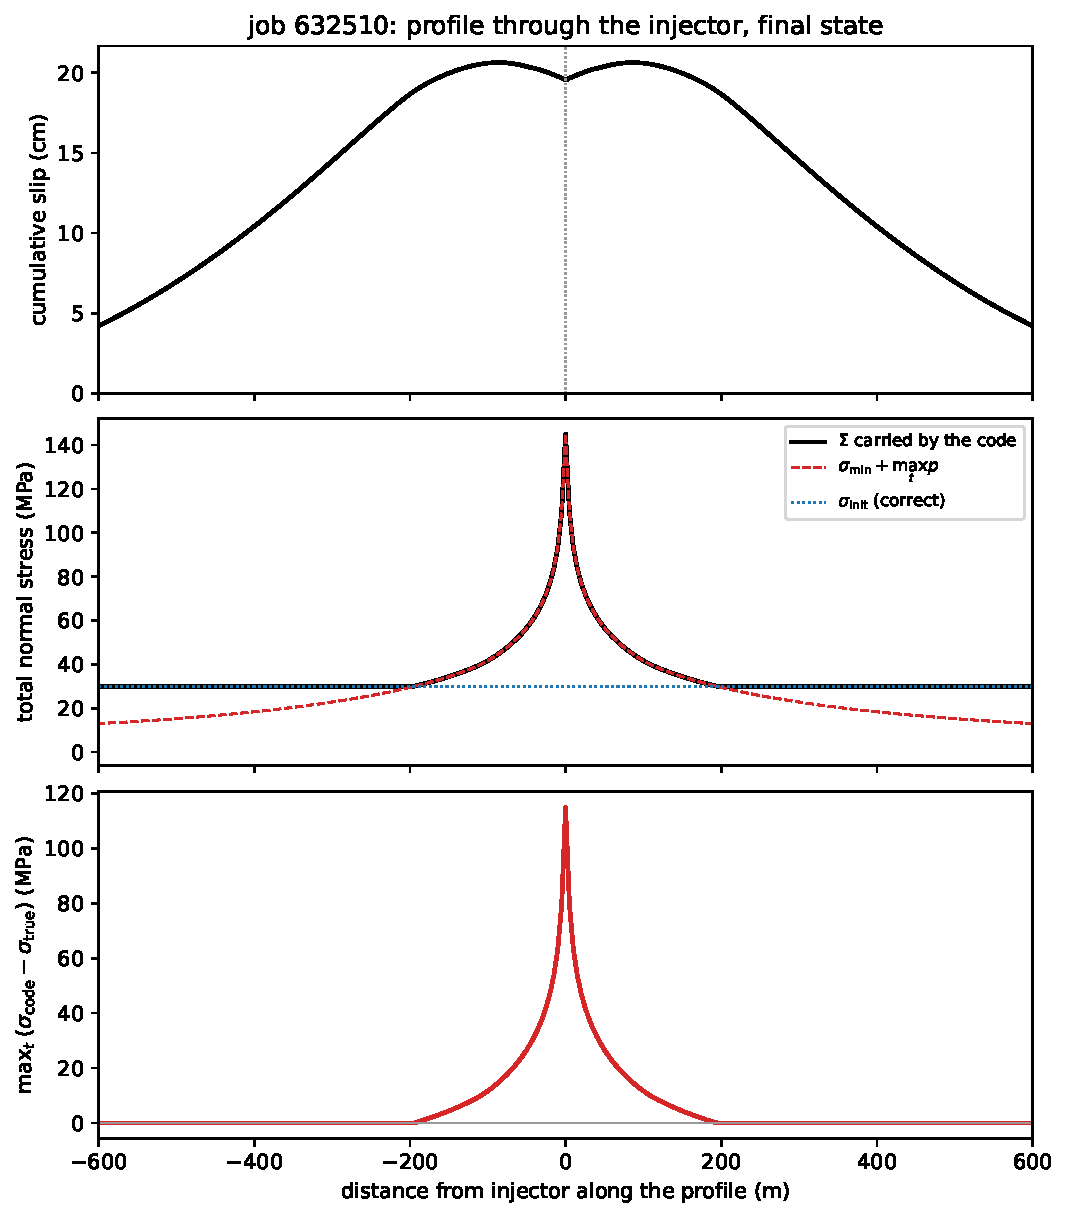
\includegraphics[width=0.82\textwidth]{figs/clamp_ratchet_profile_632510.pdf}
\caption{Profile through the injector at the final timestep. Top: the
cumulative-slip cusp. Middle: total normal stress carried by the code
(black) against the prediction \eqref{eq:ratchet} (red dashed) and the correct
value (blue dotted). Bottom: peak error in effective normal stress. The error
vanishes at $|r|\approx190$~m, the edge of the region where $p$ ever exceeded
$29$~MPa.}
\label{fig:profile}
\end{figure}

\subsection{Effect on slip}

Because the ratchet only manifests when $p$ \emph{falls} --- when $p$ is at
its running maximum the code and the truth agree, both sitting at
$\sigma_{\min}$ --- the injector cell is repeatedly and spuriously
strengthened during the troughs of the injection schedule. At day 0.956, for
instance, $p=91$~MPa at the injector, so the true effective normal stress is
pinned at $1$~MPa; the code instead reports $29.08$~MPa. The friction
coefficient $\tau/\sigeff$ required to sustain slip collapses, and the cell
locks: $V$ drops from ${\sim}10^{-6}$ to ${\sim}10^{-24}$~m/s while its
neighbours 85~m away continue sliding at ${\sim}10^{-7}$~m/s.

Over the run, the injector cell spends $67.5\%$ of output frames with an
effective normal stress too high by more than $0.5$~MPa; that fraction falls
to $36.8\%$ at $r=50$~m, $16.3\%$ at $r=85$~m, and $0\%$ beyond $200$~m.

\begin{figure}[h]
\centering
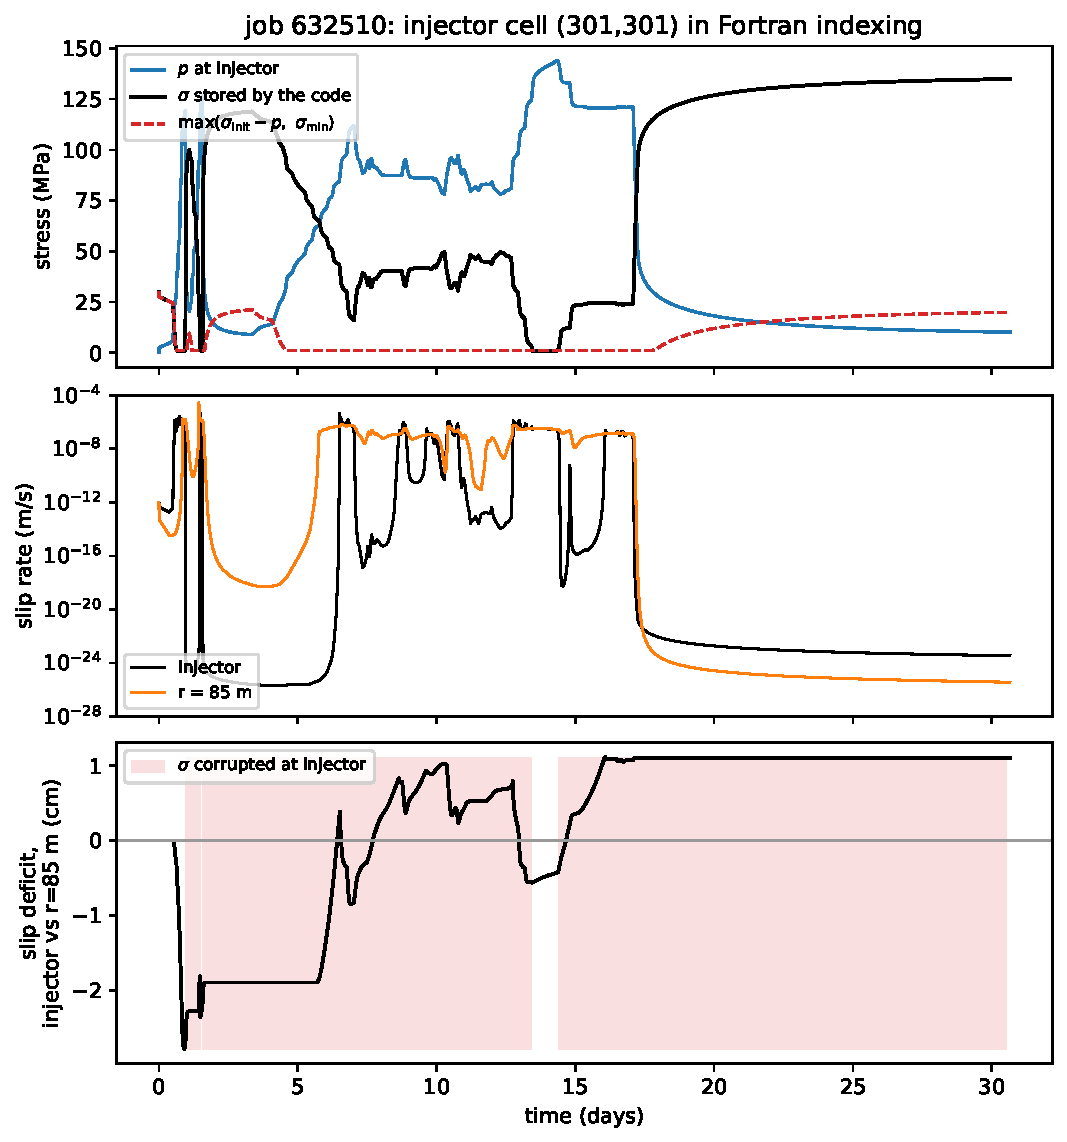
\includegraphics[width=0.82\textwidth]{figs/clamp_ratchet_history_632510.pdf}
\caption{Time histories at the injector cell. Top: pore pressure, the stored
effective normal stress, and the value required by \eqref{eq:intended}. The
two diverge from day ${\sim}1$ onward, every time $p$ recedes from a peak.
Middle: slip rate at the injector versus a cell 85~m away --- the injector
switches off entirely during the corrupted intervals. Bottom: cumulative slip
deficit between the two cells, with the corrupted intervals shaded.}
\label{fig:history}
\end{figure}

%======================================================================
\section{Why a 115 MPa error yields only a 1 cm cusp}

This is the natural objection to the diagnosis, and it is worth answering
carefully: the error in $\sigeff$ is two orders of magnitude larger than the
stress scale of the problem, yet the visible artefact in Figure~24 is about
one centimetre out of twenty.

\subsection{The error is a switch, not a forcing}

Once $\tau/\sigeff$ falls below the frictional strength, the cell is locked
and $V$ is exponentially small. It makes no difference whether $\sigeff$ is
too high by $20$~MPa or by $115$~MPa: the cell is equally dead either way. The
error therefore acts as an on/off switch on locking, and what it controls is
the \emph{duration} of the lock-ups, not their depth.

\subsection{Elasticity bounds the lag}

A patch of radius $a$ that lags its surroundings by a slip deficit $\delta$
develops a stress concentration of order
\begin{equation}
  \Delta\tau \;\sim\; \frac{\mu\,\delta}{a}.
  \label{eq:stiffness}
\end{equation}
With $\mu=24$~GPa, $a\approx100$~m and $\delta=1.1$~cm this is
$\Delta\tau\approx2.6$~MPa. The entire stress-drop budget of this problem is
about $10$~MPa (initial shear stress $\mu_{\rm init}\sigma_{\rm init} =
0.37\times30 = 11.1$~MPa, falling to ${\sim}1$~MPa in the slipped region).
A centimetre-scale deficit already consumes a quarter of that. The
surroundings then load the locked patch hard enough that it re-slips the
moment $p$ rises again and the clamp returns $\sigeff$ to $\sigma_{\min}$.
The fault simply cannot express a much larger lag.

\subsection{Direct accounting}

Splitting the growth of the injector-vs-$85$~m slip deficit by whether the
injector's normal stress was corrupted at that instant:

\begin{center}
\begin{tabular}{lr}
\toprule
Deficit accumulated while $\sigeff$ corrupted ($>0.5$~MPa error) & $+3.534$ cm \\
Deficit recovered while $\sigeff$ correct                        & $-2.429$ cm \\
\midrule
Net deficit (the depth of the cusp)                              & $+1.105$ cm \\
\bottomrule
\end{tabular}
\end{center}

So the cusp is the residual of a repeated lock/catch-up cycle: the bug injects
$3.5$~cm of deficit and elastic loading heals $2.4$~cm of it. This also
explains the shape --- the profile is smooth rather than showing a one-cell
notch, because the healing phases redistribute the lag over the whole
$190$~m clamped patch.

\subsection{The plot understates the error}

Before the ratchet takes hold (up to day ${\sim}0.9$), the injector correctly
\emph{leads} the $85$~m cell by $2.8$~cm, which is the physically expected
behaviour. The ratchet erases that lead and then reverses it. The total error
in relative slip is therefore about $4$~cm on a $20$~cm signal --- roughly
$20\%$ --- of which the figure shows only the $1.1$~cm that ended up on the
wrong side of zero.

%======================================================================
\section{Proposed fix}
\label{sec:fix}

$\sigtot$ must become a genuine state variable, advanced only by the elastic
increment and never reconstructed from a clamped $\sigeff$. The code already
uses this pattern in the analytical-injection path
(\code{main\_LH.f90:2470}, \code{sigma0(i)=sigma0(i)+y(3*i)-sigma(i)}); the
numerical-diffusion path is the one that lacks it.

Introduce one extra array, \code{sigmac}, holding the value of $\sigeff$ that
was written into \code{y} at the end of the previous diffusion step. The
difference \code{sigma(i)-sigmac(i)} is then exactly $\Delta_n$, the elastic
increment of the RK step, uncontaminated by the clamp.

\begin{enumerate}
\item Declare and allocate \code{sigmac} alongside \code{sigmat}
      (\code{main\_LH.f90:68,549}).

\item Initialise both once, in the loop that sets up \code{y} just before the
      time loop (\code{main\_LH.f90:1078--1084}); this covers the fresh-start
      and restart paths alike, since both have \code{sigma} and \code{pf}
      populated by that point:
\begin{lstlisting}[style=f90]
  do i=1,NCELL
    y(3*i-2) = psi(i)
    y(3*i-1) = tau(i)
    y(3*i)   = sigma(i)
    sigmat(i) = sigma(i) + pf(i)   ! NEW: total normal stress, a true state
    sigmac(i) = sigma(i)           ! NEW: last clamped value handed to the RK
  end do
\end{lstlisting}

\item \textbf{Delete} the per-step reconstruction at
      \code{main\_LH.f90:1124}:
\begin{lstlisting}[style=f90]
      mu(i)=tau(i)/sigma(i)
-     sigmat(i)=sigma(i)+pf(i)
\end{lstlisting}

\item Advance \code{sigmat} by the elastic increment only, in
      \code{pressure\_diffusion} (\code{main\_LH.f90:2449--2458}):
\begin{lstlisting}[style=f90]
    do i=1,ncell
      i_=st_sum%lodc(i)
      pf(i)=pfG(i_)
      dpdt(i)=(pf(i)-pfo(i))/dtdid
      sigmat(i)=sigmat(i)+(sigma(i)-sigmac(i))  ! NEW: elastic increment only
      sigma(i)=sigmat(i)-pf(i)
      if(limitsigma) then
        if(sigma(i)<minsig) sigma(i)=minsig
        if(sigma(i)>maxsig) sigma(i)=maxsig
      end if
      sigmac(i)=sigma(i)                        ! NEW: remember what we handed out
      y(3*i)=sigma(i)
    end do
\end{lstlisting}
\end{enumerate}

With this change the clamp becomes the pure projection \eqref{eq:intended}:
$e_n$ no longer enters \eqref{eq:telescope}, and for \code{3dp} the identity
$\sigeff = \max(\sigma_{\rm init}-p,\ \sigma_{\min})$ holds exactly for all
time. The guard in \code{deriv} remains consistent: when $\sigeff$ sits at the
floor, $\dot\sigtot^{\rm el}$ is zeroed, so $\Delta_n=0$ and \code{sigmat} is
correctly left unchanged.

\paragraph{Regression check.} For any \code{3dp} run, assert
$\max_i\big|\,\sigeff_i + p_i - \sigma_{{\rm init},i}\,\big| < \epsilon$ at
every output step. It should be zero to round-off, since \code{sigmaconst} is
\code{.true.} and nothing may move the total normal stress.

\paragraph{Restart caveat.} On restart, \code{sigma} is read back from
\code{output/sigma*.dat} (\code{main\_LH.f90:674--681}), so a restart from a
run made with the current code inherits whatever corruption is already in that
field. Restarted chains should be rerun from $t=0$ after the fix.

%======================================================================
\section{Implications}

\paragraph{Which results are affected.} Any run in which $p$ exceeded
$\sigma_{\rm init} - \sigma_{\min}$ anywhere on the fault. For job 632510 that
is a $190$~m radius disc around the injector --- which is the near-well region
that most of the validation figures are about. Runs where $p$ stayed below
that threshold are untouched, exactly and verifiably (Table~\ref{tab:ratchet},
bold entries).

\paragraph{A separate modelling question.} Even with the ratchet fixed, this
run drives $p$ to $144$~MPa against $\sigma_{\rm init}=30$~MPa, so everything
above $29$~MPa is discarded by the floor and the near-well effective stress is
set by $\sigma_{\min}$ rather than by the physics. That is worth discussing on
its own terms:
\begin{itemize}
\item The peak is a single 5~m cell acting as a point source, so its
      magnitude is grid-dependent; the Peaceman well index mitigates but does
      not remove this.
\item $\sigma_{\rm init}=30$~MPa with $p$ reaching several times that is
      outside the regime where a floored-$\sigeff$ model is meaningful. If
      the fault genuinely reaches $\sigeff\to0$, the physical treatment is
      \code{opening T} (which also turns the normal kernel back on), not a
      numerical floor.
\item Alternatively the injection schedule, wellbore storage $S_w$, or
      $k_{\min}$ may need revisiting so that $p$ stays below
      $\sigma_{\rm init}$.
\end{itemize}

\paragraph{The figure itself is fine.} The cusp is present in the raw
\code{slip632510.dat}; cell 85 of
\code{cooper\_basin\_\allowbreak validation\_\allowbreak stage\_\allowbreak june15.ipynb} cuts through
$j=\lfloor j_{\max}/2\rfloor = 300$, which is the injector column, and
reproduces the binary data faithfully. One cosmetic note: cell 85 labels the
$i$ axis ``down-dip'' while cell 86 fixes $i$ and sweeps $j$ under the same
label. The geometry is symmetric here so nothing follows from it, but the two
cells disagree about which index is down-dip.

\end{document}
